\normalfalse \difficiletrue \tdifficilefalse
\correctionfalse

%\UPSTIidClasse{11} % 11 sup, 12 spé
%\newcommand{\UPSTIidClasse}{11}

\exer{Détermination des efforts dans une structure étayée  $\star\star$ \label{C2:07:515}}
\setcounter{numques}{0}
\UPSTIcompetence[2]{C2-07}
\index{Compétence C2-07}
\index{PFS}
\ifcorrection
\else
\textbf{Pas de corrigé pour cet exercice.}
\fi


\ifprof
\else
Lors de la démolition d'une partie de la gare de Lyon Part-Dieu (en 2018), des étais ont du être posés afin de soutenir la structure supérieure. 

\begin{center}
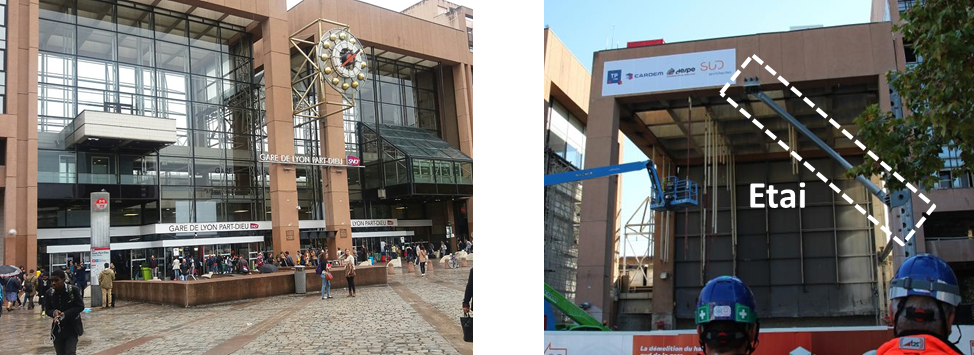
\includegraphics[width=\linewidth]{515_03}
%\textit{}
\end{center}

Dans le but de dimensionner les étais, il est nécessaire de déterminer les actions mécanique dans chacune des liaisons. 

Pour cela, on utilise la modélisation suivante. 

\begin{center}
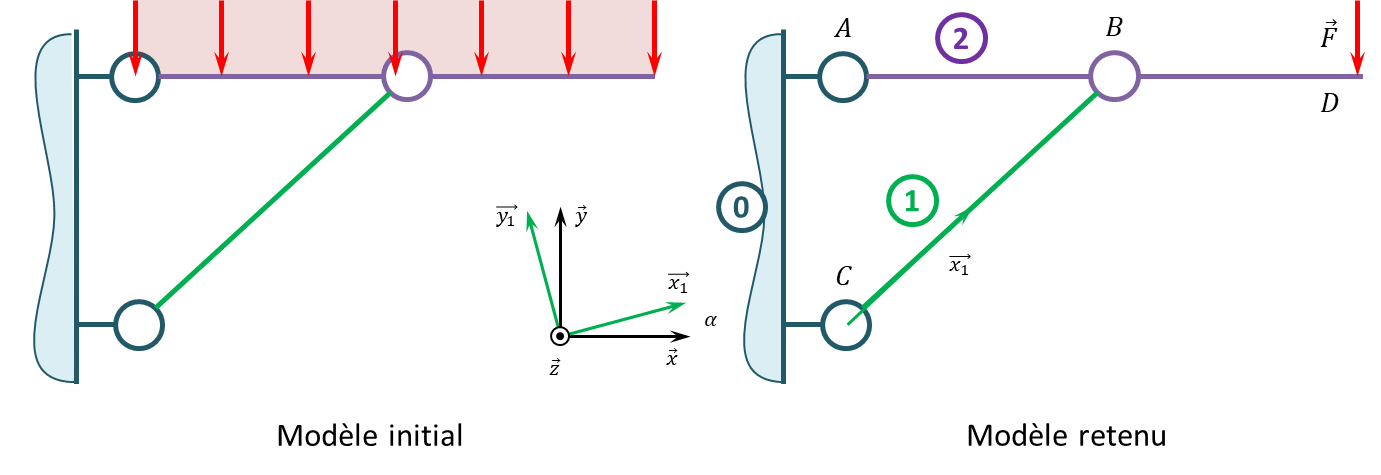
\includegraphics[width=\linewidth]{515_04}
%\textit{}
\end{center}

On a $\vect{AB}=a \vect{x}$,  $\vect{BD}=b \vect{x}$ et  $\vect{CB}=L \vect{x_1}$.
\fi

\question{Tracer le graphe d'analyse du système (graphe des liaisons et actions extérieures).}
\ifprof
\begin{corrige}
\begin{center}
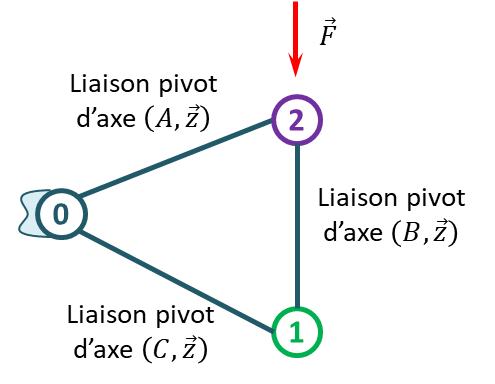
\includegraphics[width=\linewidth]{515_cor_01}
%\textit{}
\end{center}

\end{corrige}
\else
\fi

\question{Proposer une stratégie permettant de déterminer les actions mécaniques dans les liaisons.}
\ifprof
\begin{corrige}
Ici, il s'agit de déterminer les actions mécaniques dans toutes les liaisons. Il faudra donc isoler successivement toutes les pièces et réaliser un PFS pour chacune d'entre elles. Cependant, il y a quand même une stratégie d'isolement à avoir : \textbf{il faut commencer par isoler les solides soumis à deux glisseurs}. En effet, d'après le PFS, lorsqu'un solide est soumis à deux glisseurs, les deux forces sont de même norme, de même direction (droite passant par le point d'application des deux glisseurs) et de sens opposé. 

La stratégie est donc la suivante : 
\begin{itemize}
\item on isole 1 et on réalise le PFS. 
\item on isole 2 et on réalise le PFS en B. 
\end{itemize} 


\end{corrige}
\else
\fi


\question{Déterminer les actions mécaniques dans les liaisons en fonction de $F$.}
\ifprof
\begin{corrige}

\textbf{On isole 1}.
\textbf{On réalise le BAME :}
\begin{itemize}
\item $\torseurstat{T}{0}{1}$;
\item $\torseurstat{T}{2}{1}$.
\end{itemize}
\textbf{D'après le PFS pour un solide soumis à 2 glisseurs, on a : }
$\torseurstat{T}{0}{1} + \torseurstat{T}{2}{1} = {0}$. 

\textbf{Résolution :} 
$ \torseurstat{T}{0}{1} = -\torseurstat{T}{2}{1}  = \torseurl{F_{01}\vect{x_1}}{\vect{0}}{A}$.

\end{corrige}

\begin{corrige}

\textbf{On isole 2}.
\textbf{On réalise le BAME :}
\begin{itemize}
\item $\torseurstat{T}{0}{2} =\torseurl{X_{02}\vect{x} +Y_{02}\vect{y}  }{\vect{0}}{A} $ $=\torseurl{X_{02}\vect{x} +Y_{02}\vect{y}  }{-aY_{02}\vect{z}}{A} $;
\item $\torseurstat{T}{1}{2} = \torseurl{F_{01}\vect{x_1}  }{\vect{0}}{B} $;
\item $\torseurstat{T}{\text{ext}}{2} = \torseurl{-F\vect{y}  }{\vect{0}}{C} $ $= \torseurl{-F\vect{y}  }{-Fb\vect{z}}{C}$.
\end{itemize}
\textbf{D'après le PFS pour un solide soumis à 2 glisseurs, on a : }

$\torseurstat{T}{0}{2} + \torseurstat{T}{1}{2}+\torseurstat{T}{\text{ext}}{2} = {0}$.

 \textbf{Résolution :}

$\left\{ \begin{array}{l}
X_{02}+F_{01}\cos\alpha  = 0 \\
Y_{02}+F_{01}\sin\alpha  -F= 0 \\
-aY_{02}-Fb  = 0 \\
\end{array}
\right.$


$
\Leftrightarrow 
\left\{ \begin{array}{l}
X_{02}=-F_{01}\cos\alpha  =-F\dfrac{a+b}{a\tan\alpha} \\
F_{01}  =\dfrac{F-Y_{02}}{\sin\alpha}=F\dfrac{a+b}{a\sin\alpha} \\
Y_{02} = -\dfrac{b}{a}F  \\
\end{array}
\right.$

\end{corrige}

\else
\fi



\ifprof
\else

\noindent\footnotesize
\fbox{\parbox{.9\linewidth}{
Éléments de corrigé : 
\begin{enumerate}\setcounter{enumi}{2}
    \item $X_{02}=-F\dfrac{a+b}{a\tan\alpha}$, $F_{01}  =F\dfrac{a+b}{a\sin\alpha}$, $Y_{02} = -\dfrac{b}{a}F$.
\end{enumerate}}}
\normalsize


\begin{flushright}
\footnotesize{Corrigé  voir \ref{C2:07:515}.}
\end{flushright}%
\fi